\documentclass[tikz,border=12pt]{standalone}
\usepackage{fontspec}
\setmainfont{Segoe UI}
\usepackage{amsmath,amssymb}
\usepackage{tikz}

\usetikzlibrary{calc,arrows.meta}

\begin{document}
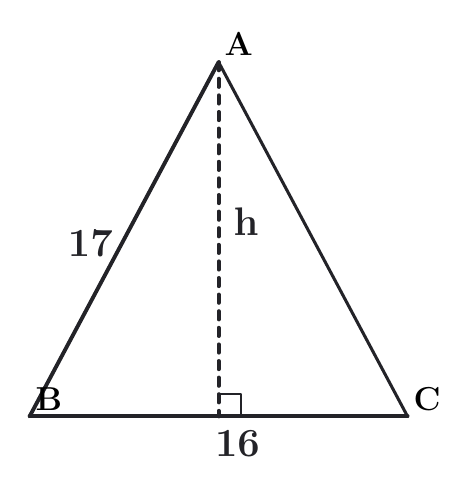
\begin{tikzpicture}[x=1.0000cm,y=1cm,line cap=round,line join=round]
\definecolor{linec0}{RGB}{35,35,40}
\definecolor{linec1}{RGB}{35,35,40}
\definecolor{linec2}{RGB}{35,35,40}
\definecolor{linec3}{RGB}{35,35,40}
\definecolor{linec4}{RGB}{35,35,40}
\definecolor{linec5}{RGB}{35,35,40}
\definecolor{edgecol}{RGB}{35,35,40}
\definecolor{hicol}{RGB}{35,35,40}
\definecolor{angcol}{RGB}{35,35,40}
\coordinate (A) at (0.0000,4.5000);
\coordinate (B) at (-2.4000,0.0000);
\coordinate (C) at (2.4000,0.0000);
\coordinate (H) at (0.0000,0.0000);
\draw[line width=1.4pt,color={rgb,255:red,35;green,35;blue,40}] (A) -- (B);
\draw[line width=1.4pt,color={rgb,255:red,35;green,35;blue,40}] (B) -- (C);
\draw[edgecol,line width=1.1pt] (C) -- (A);
\draw[line width=1.4pt,color={rgb,255:red,35;green,35;blue,40},dashed] (A) -- (H);
\draw[edgecol,line width=0.7pt] (0.000,0.280) -- (0.280,0.280) -- (0.280,0.000);
\node[font=\bfseries\Large,text={rgb,255:red,35;green,35;blue,40}] at (-1.629,2.190) {17};
\node[font=\bfseries\Large,text={rgb,255:red,35;green,35;blue,40}] at (0.240,-0.350) {16};
\node[font=\bfseries\Large,text={rgb,255:red,35;green,35;blue,40}] at (0.350,2.475) {h};
\node[font=\bfseries\large,inner sep=2pt,anchor=south west] at (0.000,4.500) {A};
\node[font=\bfseries\large,inner sep=2pt,anchor=south west] at (-2.400,0.000) {B};
\node[font=\bfseries\large,inner sep=2pt,anchor=south west] at (2.400,0.000) {C};
\end{tikzpicture}
\end{document}
